\documentclass[11pt,french,a4paper]{article}
\usepackage[utf8]{inputenc}
\usepackage[french]{babel}
\usepackage[T1]{fontenc}
\usepackage{fancyhdr}
\usepackage{lastpage}
\usepackage{fancybox}
\usepackage{graphicx}
\usepackage{appendix}
\usepackage[left=2cm,right=2cm,top=2cm,bottom=2.5cm]{geometry}
\geometry{a4paper}
\setlength{\parindent}{0pt}
\usepackage{listings}
\usepackage{color}
\usepackage[table]{xcolor}
\usepackage{array}
\usepackage{listings}
\usepackage{hyperref}
\usepackage{caption}
\usepackage{lastpage}
\pagestyle{fancy}

\definecolor{darkWhite}{rgb}{0.94,0.94,0.94}

\lstset{
  aboveskip=3mm,
  belowskip=-2mm,
  backgroundcolor=\color{darkWhite},
  basicstyle=\footnotesize,
  breakatwhitespace=false,
  breaklines=true,
  captionpos=b,
  commentstyle=\color{red},
  deletekeywords={...},
  escapeinside={\%*}{*)},
  extendedchars=true,
  framexleftmargin=16pt,
  framextopmargin=3pt,
  framexbottommargin=6pt,
  frame=tb,
  keepspaces=true,
  keywordstyle=\color{blue},
  language=C,
  literate=
  {²}{{\textsuperscript{2}}}1
  {⁴}{{\textsuperscript{4}}}1
  {⁶}{{\textsuperscript{6}}}1
  {⁸}{{\textsuperscript{8}}}1
  {€}{{\euro{}}}1
  {é}{{\'e}}1
  {è}{{\`{e}}}1
  {ê}{{\^{e}}}1
  {ë}{{\¨{e}}}1
  {É}{{\'{E}}}1
  {Ê}{{\^{E}}}1
  {û}{{\^{u}}}1
  {ù}{{\`{u}}}1
  {â}{{\^{a}}}1
  {à}{{\`{a}}}1
  {á}{{\'{a}}}1
  {ã}{{\~{a}}}1
  {Á}{{\'{A}}}1
  {Â}{{\^{A}}}1
  {Ã}{{\~{A}}}1
  {ç}{{\c{c}}}1
  {Ç}{{\c{C}}}1
  {õ}{{\~{o}}}1
  {ó}{{\'{o}}}1
  {ô}{{\^{o}}}1
  {Õ}{{\~{O}}}1
  {Ó}{{\'{O}}}1
  {Ô}{{\^{O}}}1
  {î}{{\^{i}}}1
  {Î}{{\^{I}}}1
  {í}{{\'{i}}}1
  {Í}{{\~{Í}}}1,
  morekeywords={*,...},
  numbers=left,
  numbersep=10pt,
  numberstyle=\tiny\color{black},
  rulecolor=\color{black},
  showspaces=false,
  showstringspaces=false,
  showtabs=false,
  stepnumber=1,
  stringstyle=\color{gray},
  tabsize=4,
  title=\lstname,
}

\fancyhead[L]{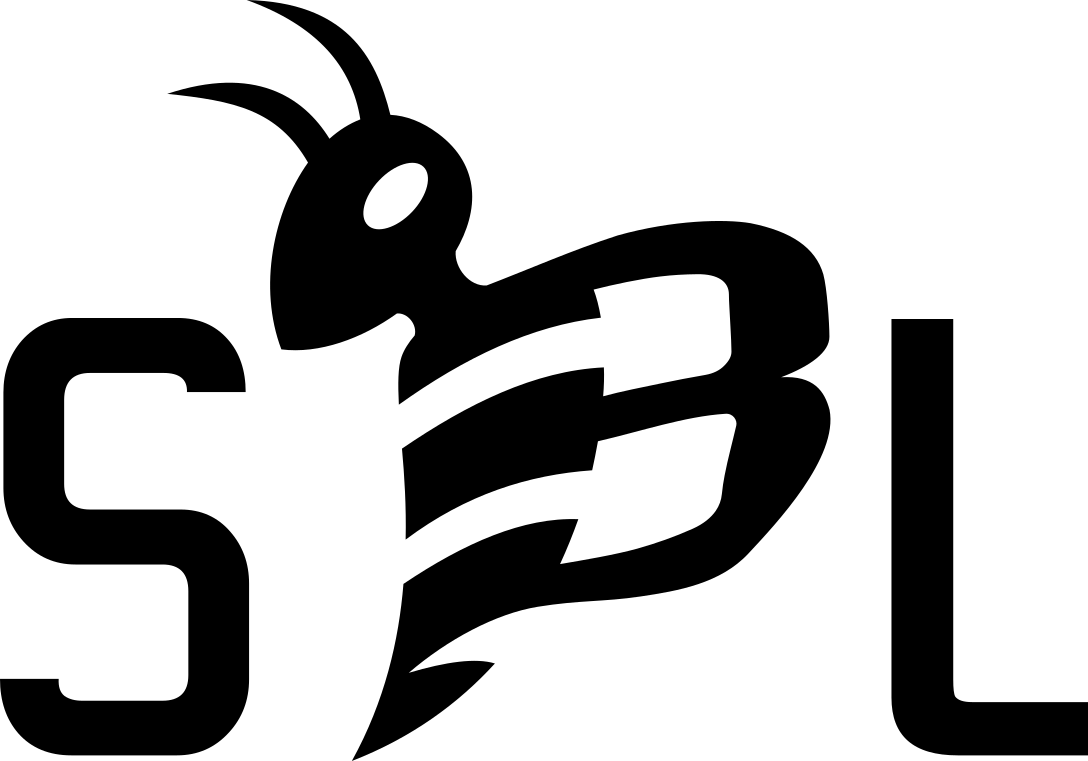
\includegraphics[width=1cm]{../../../logo/SBLlogo.png}}
\fancyhead[C]{Rapport d'activités mois de mai 2022 }
\fancyhead[R]{ 
\includegraphics[width=1.2cm]{../../../logo/IUTlogo.png}}
\fancyfoot[L]{\small Tom TUELEAU\normalsize}
\fancyfoot[C]{}
\fancyfoot[R]{\thepage/\pageref{LastPage}}


\lstset{
  basicstyle=\fontfamily{lmvtt}\selectfont\small,
  columns=fullflexible,
}

\title{
 \centering
         
\includegraphics[width=4cm]{../../../logo/IUTlogo.png}  \hspace{7cm}
         
\includegraphics[width=4cm]{../../../logo/UMlogo.png}  \hspace{7cm}
    
	\LARGE{Rapport d'activités mensuel}
	\author{TUELEAU Tom}
}
\author{
	\date{}
}
\begin{document}
\maketitle
	 
\includegraphics[width=4cm]{../../../logo/LIRMMlogo.png}  \hspace{7cm}
         \includegraphics[width=4cm]{../../../logo/IBMMlogo.jpg}  \hspace{7cm}
\newpage
\tableofcontents
\newpage
\section{Introduction}
Ce document a pour objectif de faire un état d'avancement du stage. Celui-ci résumera donc le travail fait lors de la fin du mois d'avril et le mois de mai.
\\Dans un premier temps, je reviendrai sur le montage amplificateur vu lors du dernier rapport et vous exposerai les résultats obtenus.
\\Une seconde partie présentera les programmes créés afin de récolter, envoyer et traiter les données des capteurs. 
\\Enfin, je conclurai sur le travail effectué et les difficultés rencontrées. 

\section{Finalisation du montage}
Lors des précédents rapports\footnote{Voir "Rapport d’activités du 11 et 18 avril 2022", partie 4, page 7}, je vous ai exposé mes recherches et résultats quand au dimensionnement d'un montage amplificateur. Ce besoin s'était fait ressentir quand je m'étais rendu compte que le signal émis par le piézo-électrique n'arrivait pas à être capté par l'Arduino.  Dans cette partie nous verrons tout d'abord la finalisation du montage et dans un second temps nous verrons l'installation de celui-ci dans le rucher.\\
\subsection{Montage}
Lors de cette semaine j'ai pu effectuer le prototype incluant l'amplification du signal, le piézo-électrique, le capteur de température et d'humidité (Si7021) et l'Arduino. Vous pouvez voir un schéma complet Figure \ref{SMG}.
\\
\begin{center}
    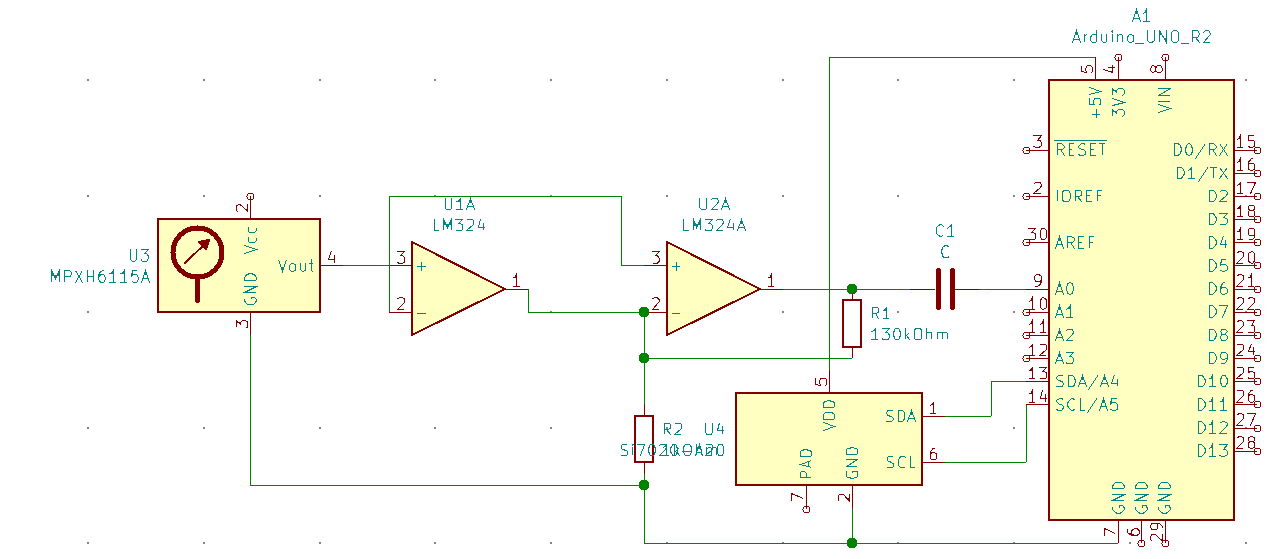
\includegraphics[scale=0.5]{../img/SMG.png}
    \captionof{figure}{Schéma montage final}
    \label{SMG}
\end{center}
Comme nous le verrons lors de la partie programmation, j'arrive à récupérer le signal envoyé par le piézo-électrique avec l'Arduino. Cela va donc me permettre d'échantillonner celui-ci et de le traiter.
\subsection{Installation dans la ruche}
L'objectif étant de récolter les données dans la ruche, j'ai du installer les capteurs dans celle-ci. Comme vous pouvez le voire Figure \ref{RC}, j'ai glissé les différents capteurs dans la ruche et leur ai soudé des fils assez longs pour les brancher par la suite sur un microcontrôleur.

\begin{center}
    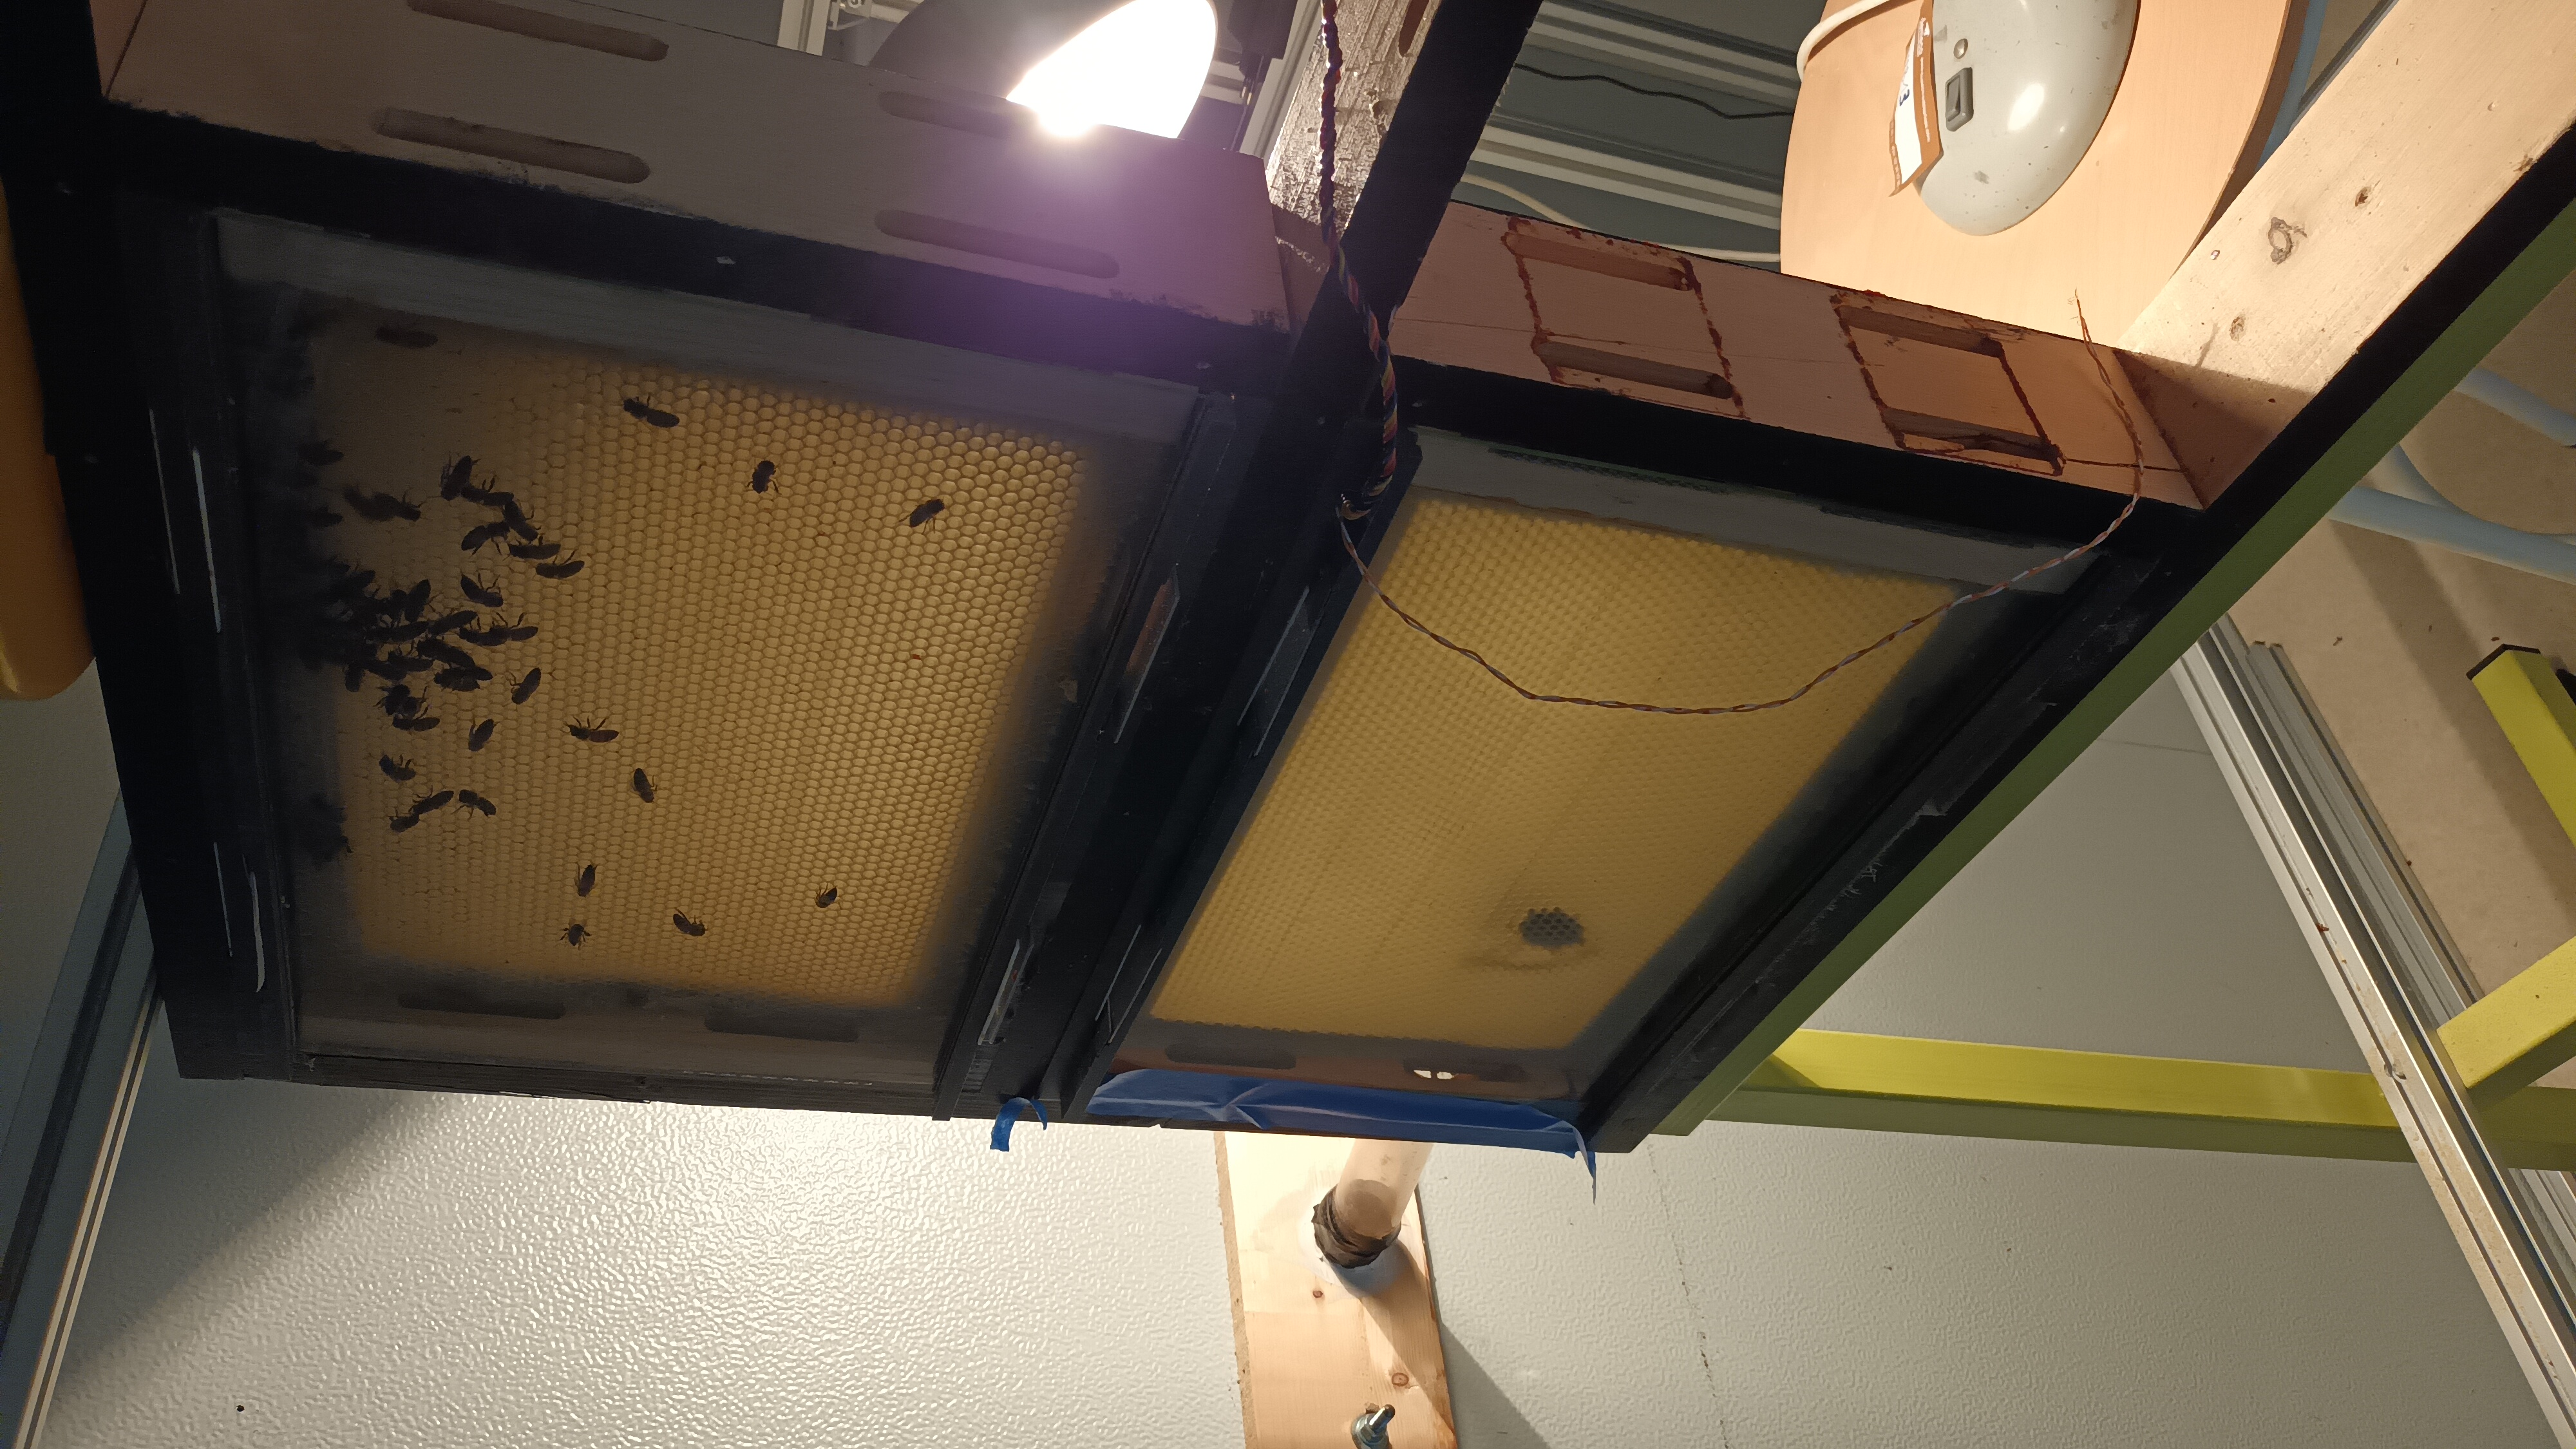
\includegraphics[scale=0.1,angle=270]{../img/RC.png}
    \captionof{figure}{Capteurs dans la ruche}
    \label{RC}
\end{center}
Le montage est maintenant installé dans la ruche, il reste cependant à installer un câble Ethernet afin de relier l'Arduino au réseau.
\subsection{Résultats}
Après avoir échantillonné le signal obtenu par le piézo-électrique et l'avoir envoyé au serveur de traitement, j'ai pu obtenir le graphique Figure \ref{G1}\footnote{ Abscisse : temps en ms Ordonnée : tension en V }.
\begin{center}
    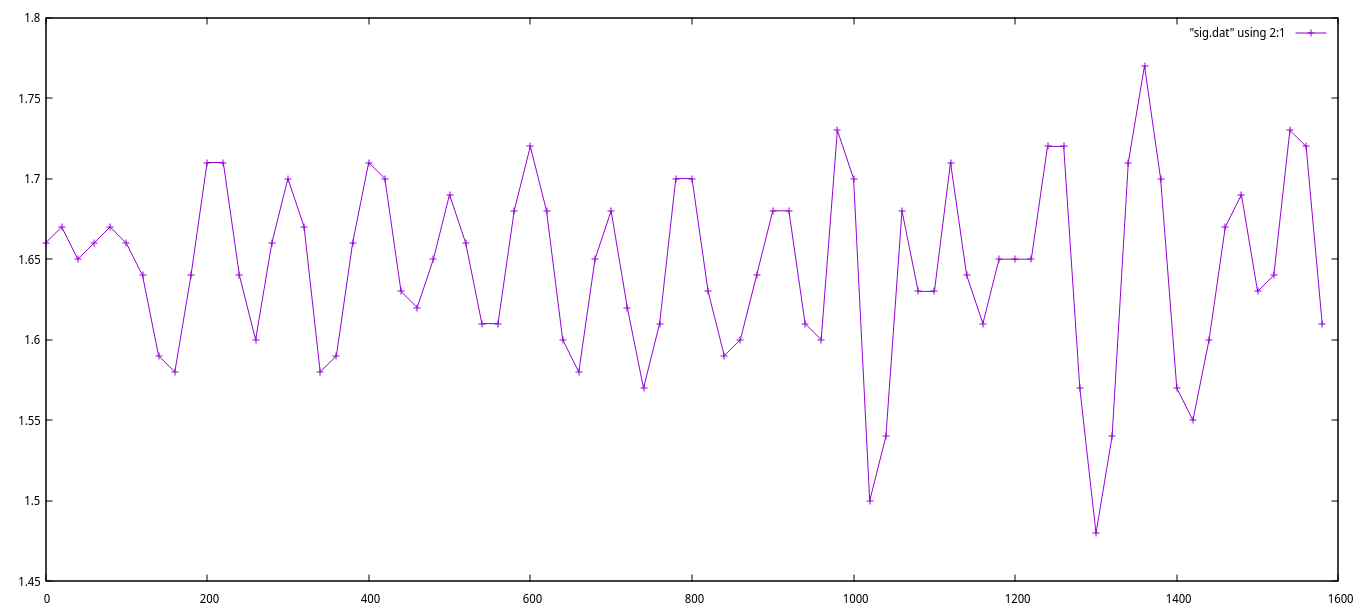
\includegraphics[scale=0.3]{../img/GRAPH1.png}
	\captionof{figure}{Graphique du signal piézo-électrique}
    \label{G1}
\end{center}
\subsection{Améliorations}
Maintenant que ce montage est fonctionnel, j'aimerais pouvoir lui apporter des améliorations. La première serait la création d'un PCB pour le montage amplificateur afin de rendre le montage plus professionnel. La seconde serait la création d'un boitier pouvant le contenir lui et l'Arduino. 
\newpage
\section{Programmation}
Tout au long des dernières semaines, j'ai eu à programmer plusieurs fonctionnalités. Dans cette partie je vais donc commencer par vous présenter les programmes réalisés pour récolter les données des capteurs et effectuer leur traitement. Une deuxième partie abordera la programmation de la mise en communication des différents composants du système.
\subsection{Programmation des capteurs}
Pour ma premier mission j'avais trois  données à récupérer. Celle-ci sont l'humidité, la température et les vibrations. Afin de récolter ces données j'ai choisi en tout trois capteurs. Un capteur piézo-électrique , un capteur de température et d'humidité (Si7021) et un microphone (INMP441). Dans un premier temps je vous parlerai du capteur de température et d'humidité. Une seconde partie abordera la programmation du capteur de vibration. Enfin une derniere partie abordera le traitement des données.  

\subsubsection{Capteur de température et humidité}
Comme indiqué précédemment le capteur utilisé pour ces données est le Si7021. Étant donné que le microcontroleur que j'utilise est un Arduino, il existe des librairies donnant accès à des fonctions permettant d'obtenir les données voulues.
Les fonctions principals de ce programme sont , "sensor.begin" qui initialise la liaison entre l'Arduino et le capteur, "readHumidity" et "readTemperature" permettent comme leur nom l'indique de récupérer la température et l'humidité mesurées par le capteur. Les valeurs retourner par ces deux fonctions sont de type "double". Afin de pouvoir les envoyer, je les convertis en chaines de caractères à l'aide de la fonction "dtostrf".

\subsubsection{Capteur de vibration}
Après avoir amplifié le signal du piézo-électrique, j'ai pu me consacrer à l'acquisition des données de celui-ci. Afin de faciliter son acquisition j'ai créé une fonction "udpSendVibration" prenant la quantité d'échantillon souhaitée, le nombre de décimales et la période d'échantillonage (en milliseconde).

\begin{scriptsize}
\begin{lstlisting}

void udpSendVibration(int nbEchantillon, int nbVirgule, int periodeEchantillonageMs)
{

	int nbChar = nbVirgule+2;
	char tmp[nbEchantillon][nbChar];
	char data2[nbEchantillon*nbChar];
	double centsValeurs[nbEchantillon];
	int i,y;
	for(i=0;i<nbEchantillon;i++){
		centsValeurs[i]=analogRead(piezo);
		centsValeurs[i]=(centsValeurs[i]*5)/1023;
		delay(periodeEchantillonageMs);
	}
	delay(2000);
	for(i=0;i<nbEchantillon;i++){
		dtostrf(centsValeurs[i],nbChar,nbVirgule,tmp[i]);
		for(y=0;y<nbChar;y++){
			data2[(nbChar*i)+y]=tmp[i][y];
			Serial.println(data2[(i*nbChar)+y]);	
		}	
	}

}
\end{lstlisting}
\end{scriptsize} 

\subsubsection{Traitement des données}
Une fois le signal obtenu il fallait l'annalyser. J'avais dans un premier temps commencé à traiter les données directement sur l'Arduino en effectuant une transformé de Fourrier du signal. Cependant les capacités de calcul de l'Arduino étant limitées et ayant observé une certaine lenteur à effectuer cette opération j'ai décidé d'effectuer le systéme suivant. J'envoie les échantillons à un ordinateur distant qui effectuera le traitement et renvoie le résultat obtenu en MQTT.\\
J'ai donc par la suite écrit un programme utilisant la librairie "fftw". Celle-ci proposant de multiples fonctions bassées sur l'algorithme FFT (Fast Fourier Transform), permettant d'effectuer une transformée de Fourrier sur les signaux numérisés.

\begin{scriptsize}
\begin{lstlisting}

	unsigned int N = 20;
	int i;
	double *out = malloc(sizeof(double) * N);
	double list[]={3.920000,0.160000,5.630000,4.750000,0.370000,2.010000,
	5.870000,6.730000,9.870000,4.340000,9.950000,5.460000,8.420000,3.120000,
	3.670000,4.870000,3.280000,6.050000,4.650000,0.500000};
	double * values;
	values = malloc(sizeof(double)*N);
	fftw_plan p;
	p = fftw_plan_r2r_1d(N,values,out,FFTW_HC2R,FFTW_MEASURE);
	
	for(i=0;i<20;i++){
			values[i]=list[i];
	}
	
	fftw_execute(p);
	for(i=0;i<20;i++){
			printf("%f ",out[i]);
	}
	printf("\n");
	fftw_destroy_plan(p);
	free(out);
\end{lstlisting}
\end{scriptsize}


Dans l'exemple ci-dessus on effecue la transformée de Fourrier du signal composé des points de la liste.
\subsection{Programmation réseau}
Afin d'acheminer les informations jusqu'aux differents composantes (site web, serveur) j'ai eu à programmer plusieurs liaisons réseau. Je vais donc commencer par vous présenter la topologie de celui-ci avec les différent éléments le composant ainsi que leurs rôles. Dans un second temps je détaillerai la liaison MQTT reliant la base de données et l'Arduino. Une derniere partie traitera de la communication des données au serveur.
\subsubsection{Topologie du réseau}
Comme dit précédement le système est composé de plusieurs éléments. Tout d'abord l'Arduino récolte les données et les envoie aux autres composantes. La température et l'humidité sont envoyés via MQTT vers le serveur tandis que les données du piezo sont envoyées via UDP. Une fois traité ces derniers sont aussi envoyés sur un topic MQTT.
\begin{center}
    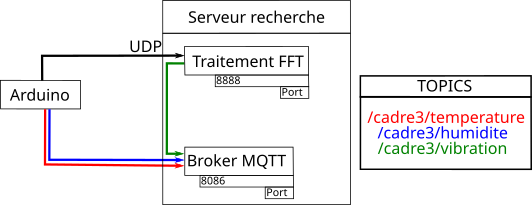
\includegraphics[scale=1]{../img/schemaNet.png}
	\captionof{figure}{Schema Réseaux}
    \label{SN}
\end{center}
\subsubsection{Liaisons MQTT}
Afin d'envoyer les données du microcontroleur vers le serveur j'ai choisi le protocole MQTT, et ce pour deux raisons. La première est que le projet sera amené à évoluer et contiendra plusieurs capteurs récoltant la même donnée à des endroits differents de la ruche. Ainsi avec le systéme de topics, on pourra identifier facilement ces différents capteurs. La deuxième est que la solution envisagée pour le site web, et la base de données, est trés facilement couplable avec ce protocole. 

\subsubsection{Liaisons UDP}
Afin de transmetre les données du piezo au serveur, j'ai choisis d'effectuer une liaisons UDP. J'ai choisi ce protocole car la liaison n'as pas besoin d'accusé de réception. L'Arduino envoie donc sur le serveur les données du piezo. Le programme ci-dessous crée une socket et attend que l'Arduino envoie ces données. 
\begin{scriptsize}
\begin{lstlisting}

	...

	int sockfd, len, n, echantillon, nbchar;
	char buffer[MAXLINE];
	struct sockaddr_in servaddr, cliaddr;
	
	if ( (sockfd = socket(AF_INET, SOCK_DGRAM, 0)) < 0 ) {
		perror("Erreur lors de la creation de la socket");
		exit(EXIT_FAILURE);
	}

	memset(&servaddr, 0, sizeof(servaddr));
	memset(&cliaddr, 0, sizeof(cliaddr));

	servaddr.sin_family = AF_INET; 
	servaddr.sin_addr.s_addr = INADDR_ANY;
	servaddr.sin_port = htons(PORT);

	if ( bind(sockfd, (const struct sockaddr *)&servaddr,sizeof(servaddr)) < 0 )
	{
		perror("bind failed");
		exit(EXIT_FAILURE);
	}

	len = sizeof(cliaddr); //len is value/result
	for(;;){
		n = recvfrom(sockfd, (char *)buffer, MAXLINE,MSG_WAITALL, ( struct sockaddr *) &cliaddr,&len);
		buffer[n] = '\0';
		sendto(sockfd, "ACK", strlen("ACK"),MSG_CONFIRM, (const struct sockaddr *)&cliaddr,sizeof(cliaddr));
	
	}

	...
\end{lstlisting}
\end{scriptsize}
\section{Conclusion}
Lors de ces semaines de travail j'ai rencontré plusieurs difficultés. Tout d'abord l'envoie et l'acquisition des données envoyées par le piézo-éléctrique furent complexe dans un premier temps. Ce problème était imputable à l'Arduino que j'utilisais dont les broches analogiques était defaillantes. La deuxième difficutlée fût sur l'utilisation de la librairie fft. En effet certains détails m'avaient échappés lors de ma première lecture de la librairie.
En conclusion, maintenant que les données ont été récoltées et acheminées il faut pouvoir les afficher sur un site web. Il me reste aussi à effectuer un montage final plus propre pour la partie electronique du système. 
\newpage
\listoffigures

\end{document}
